\documentclass[11pt]{amsart}
%%% WARNING: Do NOT change the page size, fonts, or margins!  Penalties will apply.


\usepackage{graphicx, hyperref}
\usepackage{amssymb,amsmath,amsthm, mathtools}
\usepackage{placeins} %enables \FloatBarrier, that prevents floats from going below it.
\usepackage{caption}
\usepackage{subcaption}
\usepackage{algpseudocode, algorithm}
\usepackage{tikz}
\usepackage{physics}
\usepackage[T1]{fontenc}
\usepackage{DejaVuSansMono}
\usetikzlibrary{arrows}
\usetikzlibrary{tikzmark}
\usepackage{listings}

% Define style for Python code snippets
\lstset{
    language=Python,
    basicstyle=\small\ttfamily, % Set font size to small
    frame=single, % Add frame around code snippets
    showstringspaces=false % Don't show spaces in strings
}

%%% WARNING: Do NOT change the page size, fonts, or margins!  Penalties will apply.
%%% WARNING: Do NOT change the page size, fonts, or margins!  Penalties will apply.

% Some macros for ease of use
\newcommand{\R}{{\mathbb R}}
\newcommand{\A}{{\mathrm{A}}}


\begin{document}

\title{Angle approximation from pressure measurements}
\author{Cannon Tuttle, Curtis Evans, Spencer Ashton, Tyler Sanders}

%% comment out next command to put today's date after names of group members, or put a desired day in the parethesis
\date{}

\maketitle

\begin{abstract}
    This paper attempts to adapt linear filtering methods to work with angular data in order to predict angle of arrival of human voices. The data used for this project was both simulated and real data. We used various Bayesian filtering techniques on a continuous state space model to optimize angle estimation.
\end{abstract}

%% First Section
\section{Problem Statement and Motivation}
A BYU Acoustics research project seeks to reproduce the filtered sound signal from a source near heavy machinery, within the cab for the operator. In essence, 
the machine operator should hear the reproduced voice of someone outside the cab speaking clearly from the direction they stand in relation to the machine. This 
will augment the safety of those outside the machinery by increasing the awareness of the machine operators. Our aim is to improve the robustness of the angle 
estimation in order to allow the researchers to more accurately reproduce the sound directionality.

\begin{figure}
\includegraphics*[width=0.95\textwidth]{Pic of Real Mic Array.jpg}\hfill
\caption{Microphone array used in data collection.}
\label{fig:array}
\end{figure}

Currently, the angle in relation to the center of the microphone array (see Figure \ref{fig:array}) is calculated using triangulation. Somewhat rudimentary filtering has been implemented to 
improve stability, but so far the results of the calculation are still unreliable. We modeled the angle of arrival evolution process as a continuous state space 
hidden Markov model and employed various Bayesian filtering techniques in order to optimize the angle estimation. This included adapting filters normally used 
with data defined for all real numbers and gaussian distributed noise to circular data that are defined on $[0,2\pi]$ with the wrapping property at the boundary.

Previous work has shown that an unmodified Kalman Filter does not work well on angular data, and our experience working with this data supports that conclusion. 
Various distributions, including a wrapped normal distribution and the Von Mises distribution have been adapted to be used with the Kalman Filter successfully. 
However, these adaptations are complex and not easily implemented, as they include approximating the distributions with a wrapped Dirac mixture \cite{Research}. Particle filters 
are a type of filtering algorithm that allow for the use of an arbitrary distribution and have been used with circular distributions before.



%% Second Section
\section{Data}
The data used for this project was both stimulated data and real data given to us by the research
team. The research team didn’t provide all the data we needed to test our methods, so we decided to
stimulate our own data. The situations we needed to test were a stationary angle, moving angle, and
discontinuous angle. The stationary angle would be someone standing still talking to the machine
operator, the moving angle would be someone walking around the machine while talking continuously,
and the discontinuous angle would be someone walking around the machine while talking
intermittently. The first situation we got data from the research team and the later two situations
we needed to stimulate. We are waiting for real data to test the last two with our methods. 


%% Third Section 
\section{Methods}
We have tried several methods to compute the hidden angle measurement. We tried the following methods...

\subsection{Leaky Filter}

The leaky filter is a simple filter that just takes the last $n$ samples and finds the average to use as the estimate of the true state. This is the filter currently being used on the project and the results have not been incredibly useful.

\subsection{State Space Model}
First we had to set up our continuous state space model. We needed angular velocity in our state space so to do that we do a finite difference approximation 
where $\theta'_t \approx \frac{\theta - \theta_{t-1}}{\Delta t}$. Now that we have angular velocity we can use it to make a simple forward Euler step in our state 
space. With the finite difference we need to save $\theta_{t-1}$ in the state space. This yields the following setup
\[\mathbf{x}_t = \begin{pmatrix*}[l]
    \theta_t \\
    \theta_{t-1} \\
    \theta'
\end{pmatrix*},\;  
F = \begin{pmatrix*}[l]
    1 & 0 & \Delta t \\
    1 & 0 & 0 \\
    \frac{1}{\Delta t} & \frac{1}{\Delta t} & 0
\end{pmatrix*},\;
H = \begin{pmatrix*}[l]
    1 & 0 & 0 \\
    \vdots & \vdots & \vdots\\
    1 & 0 & 0

\end{pmatrix*}\]
 where $H$ is of dimension $n\times3$ for $n$ observed angles. We don't have any control in our situation so our state space is
 \[\mathbf{x}_t = F\mathbf{x}_{t-1} + \mathbf{w}_t,\]
\[\mathbf{z}_t = H\mathbf{x}_t + \mathbf{v}_t\].

\subsection{Kalman Filter}
We implemented the Kalman filter from the Volume 3 Textbook \cite{V3} and Lab Manual \cite{V3 Lab Manual}. To understand how angle measurements worked in the Kalman Filter we tried it with
stimulated data done in the lab manuals and class. We discovered a problem with the update step in angle wraparound from the angles in the range of 
\[2\pi - \epsilon \leq \theta \leq 2\pi + \epsilon\] for some $\epsilon \geq 0$. We notices that the more noise we added the larged this $\epsilon$ got. 
See Figure \ref{fig:simple_kalman} to get a visual.

We discovered that the problem was occurring in the update step where \[\mathbf{\tilde{y}}_t = \mathbf{z}_t - H\mathbf{\hat{x}}_{t|t-1}.\]
A toy example would be if we are looking at an observed angle $\mathbf{z}_i = 15^{\circ}$ and a predicted angle of $(H\mathbf{x})_i = 355^{\circ}$ 
then $\mathbf{z}_i - (H\mathbf{x})_i = 15^{\circ} - 355^{\circ} = -340^{\circ}$ and we desire $20^{\circ}$. We could simply do this by noticing that $-340 \equiv 20 \pmod {360}$,
however, if we said $\mathbf{z}_i=355^{\circ}$ and $(H\mathbf{x})_i = 15^{\circ}$ then $\mathbf{z}_i - (H\mathbf{x})_i = 355^{\circ} - 15^{\circ} = 340^{\circ}$ which isn't what we want.
We want the Kalman filter to think of this difference as $-20^{\circ}$. The best way to do this was by implementing Algorithm \ref{alg:kalman} which will get us the right differenced needed by 
the correct sign so the Kalman filter can function correctly.

\begin{figure}[htp]
    \centering
    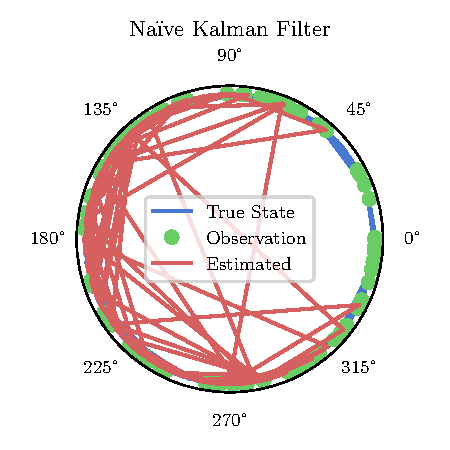
\includegraphics[width=0.47\textwidth]{non_altered_kalman.pdf}\hfill
    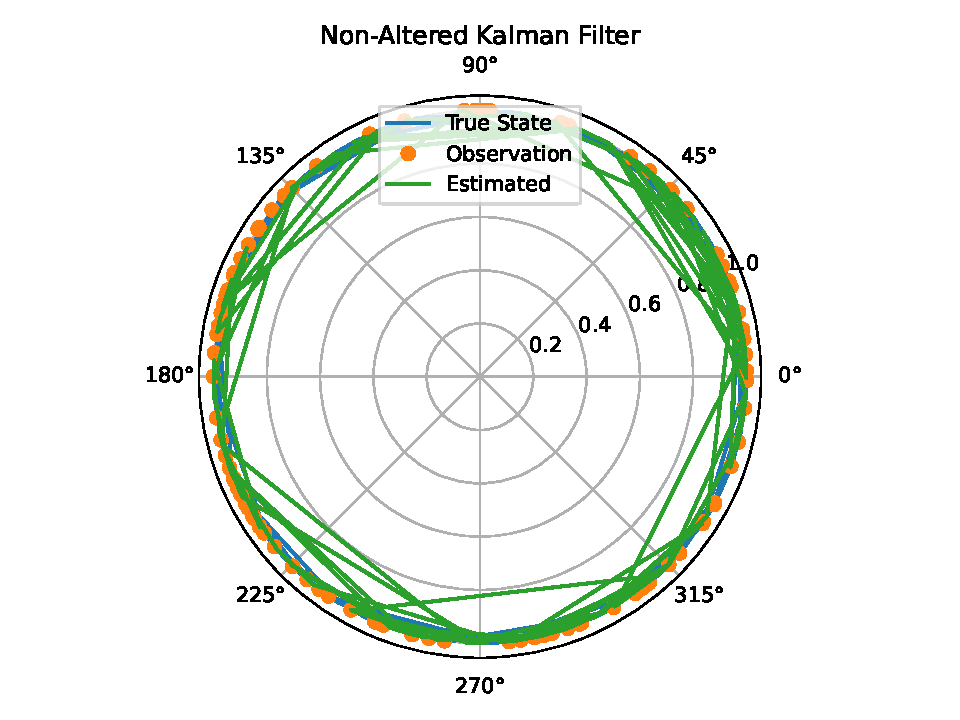
\includegraphics[width=0.47\textwidth]{altered_kalman.pdf}\hfill
    \caption{The non-altered and altered Kalman Filter}
    \label{fig:simple_kalman}
\end{figure}



\begin{algorithm}
    \caption{Process to Fix Wraparound}\label{alg:kalman}    
    \begin{algorithmic}
        \State $\mathbf{v} \gets \mathbf{z}_t - H\mathbf{x}_t$
        \If{$\lvert{\mathbf{v}}\rvert \geq \pi \;\textbf{and}\; \mathbf{v}\leq 0$} 
            \State $\mathbf{v} \gets \mathbf{v} + 2\pi$
        \ElsIf{$\lvert{\mathbf{v}}\rvert \geq \pi \;\textbf{and}\; \mathbf{v} \geq 0$} 
            \State $\mathbf{v} \gets \mathbf{v} - 2\pi$
        \EndIf 
        \State $\tilde{\mathbf{y}_t} = \mathbf{v}$ 
        \end{algorithmic}
    \end{algorithm}

%% Insert some pictures of the angle adjustment and add the algorithm 

\subsection{Particle Filter}
The second method we employed was another type of Bayesian filter, the particle filter \cite{Particle}. The particle filter employs a large number of possible current states, each referred to 
as a “particle”. Each particle has an associated weight, interpreted as the probability that particle accurately reflects the hidden state, with all weights summing to 1. As the source can possibly 
come in at any angle, we initialize the particles with uniformly distributed states and weights. At each time step, the filter propagates all of the particles forward in time according to the state space 
model, including adding state noise in the update. Then, using the data, it updates the weights of each particle by computing the posterior probabilities given data. Finally, it computes the state estimate 
as the weighted average of the states of all the particles. 

In the update step, the filter computes $P(\theta|\text{data}) \approx P(\text{data}|\theta)P(\theta)$ for each particle. The prior $P(\theta)$ is given by the particle’s previous weight, while $P(\text{data}|\theta)$ is calculated 
according to the probability distribution defined for the measurement noise. One of the benefits of the particle filter is that, unlike the normal distribution requirement of the Kalman filter, any arbitrary noise 
distribution may be employed. In this case, we used the Von Mises distribution \textcolor{red}{TODO} [DEFINE,show plot,explain Kappa parameter as it correlates to certainty on particle's location]. This closely approximates a Normal distribution 
that is “wrapped” around the angle boundary between $0$ and $2\pi$. Thus, no other consideration of angle wrapping must be made for the particle filter. After the posterior weights have been calculated, they are again normalized by 
their sum so they represent a probability distribution.

Particle filters suffer from what is called the "Degeneracy Problem", in which the weights become concentrated in a small number of the total particles. This is solved by resampling, a process in which low probability particles are replaced 
with higher probability particles. Detailing this problem and its solution is beyond our scope, but we used the \lstinline{systematic_resample} function from \lstinline{filterpy} to accomplish resampling.

As the particle filter keeps track of a large number of possible states which are distributed around the circle, it is much more flexible to nonlinear behavior. This is desirable in our case, as the source location may possibly reappear at any 
location in the state space. Unfortunately, the particle filter performs a similar number of computations for each individual particle as the Kalman filter performs in total. As we are using \lstinline{num_particles}, our particle filter takes \lstinline{n_particles} 
times as long to compute each step.

The Particle filter is defined with the following hyperparameters: 
\begin{itemize}
    \item \lstinline{K1} defines the analogous variance term for the distribution of the state noise,
    \item \lstinline{K2} defines the same for the measurements noise,
    \item \lstinline{N_particles} defines the number of particles the model employs, and
    \item \lstinline{N_eff_particles} defines the minimum number of “effective” particles allowed before particles are resampled.
\end{itemize}

Similar to the Kalman filter, we tuned the hyperparameters \lstinline{K1}, \lstinline{K2}, \lstinline{N_particles}, and \lstinline{N_eff_particles} by performing a gridsearch over many different possible values. A filter was constructed for each hyperparameter combination, with its performance 
tested across several different datasets. We then chose the hyperparameters that produced minimum average angular error over the different datasets. A similar method was implemented for a robotics research paper as well see \cite{Oops}.

\section{Results}

We had success with circular filtering techniques by using Algorithm \ref{alg:kalman} allowed us to use Kalman Filters with circular mechanics.


\section{Analysis}

TODO tradeoffs of Particle filter - the compute time 500x longer for 500 particles
- particle filter can have a more flexible prior because it's already got particles everywhere.
- particle filter better at nonlinearities bc particles can be reassigned

- Both systems have a mechanism to capture how certain they are about the current state,
- and both have a way to specify how much we "belive" current measurements

\section{Ethical Considerations}
This project seeks to augment the safety of those outside the machinery by increasing the awareness of the machine operators. However, before deployment, this model must be 
shown to improve safety as much as or more than it increased the safety perception of the operators. Risk compensation “is a theory which suggests that people typically adjust 
their behavior in response to perceived levels of risk, becoming more careful where they sense greater risk and less careful if they feel more protected” \cite{Risk}. This should 
be accounted for before deploying these methods in the field to ensure that the model performs robustly enough to truly enhance overall safety, despite risk compensation. Furthermore, 
it should be emphasized that operators should still use sight and radio communication to identify nearby individuals, and that people near machinery must still exercise caution. 

\section{Conclusion}
Our goal was to improve robustness of the angle estimation by adapting filtering methods for use with circular data. We derived a very simple modification to the Kalman filter that 
allows it to work for circular data, and we implemented a particle filter using circular probability distributions. We found the particle filter and the circular Kalman filter suitable 
for angular data. The particle filter handles nonlinearities well but comes at a computational cost, while the circular Kalman filter is computationally efficient but suffers in 
accuracy in cases of strong nonlinearity. Due to the wraparound property of angular data, the leaky filter and unmodified Kalman filter are highly unsuitable for angular data. The particle 
filter and circular Kalman filter were both suitable, and can be adapted depending on the project’s needs.

For the BYU Acoustics project specifically, if the computational cost of the filtering step is a concern, we would recommend use of the circular Kalman filter for this project due to its low 
cost and accurate performance except in cases of strong nonlinearity. If more computational headroom is allowed, the particle filter would be ideal, as it performed well even in cases of 
nonlinearities. Furthermore, the utility of these methods extends to any field in which angle measurements are taken, including robotics, navigation, and astronomy. The hyperparameters of our 
methods can easily be modified to adjust accuracy, flexibility, and computational cost depending on what is needed for the given scenario. 





\begin{figure}[htp]
    \centering
    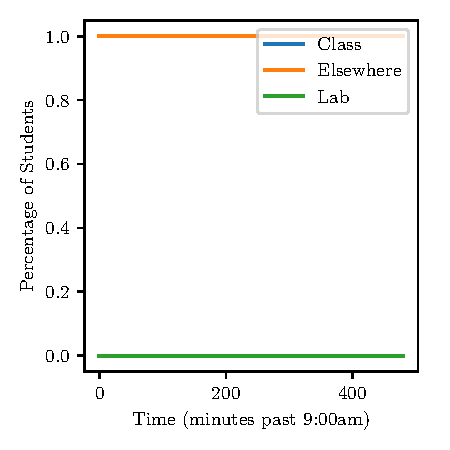
\includegraphics[width=0.45\textwidth]{temp.pdf}\hfill
    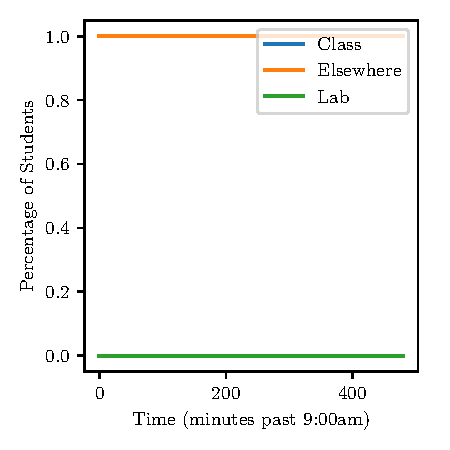
\includegraphics[width=0.45\textwidth]{temp.pdf}\hfill
    \caption{The constant alpha functions (left) along with the timeplot using IVP (right).}
    \label{fig:constant_alpha}

\end{figure}


\begin{figure}[htp]
    \centering
    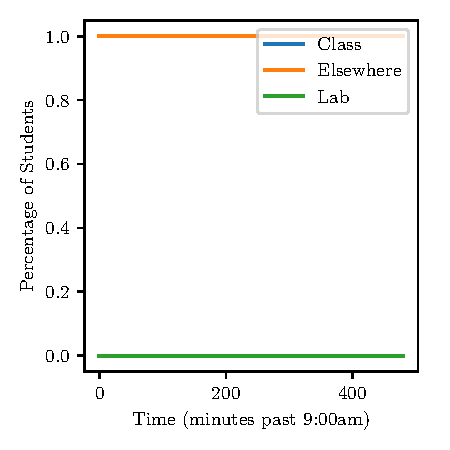
\includegraphics[width=0.45\textwidth]{temp.pdf}\hfill
    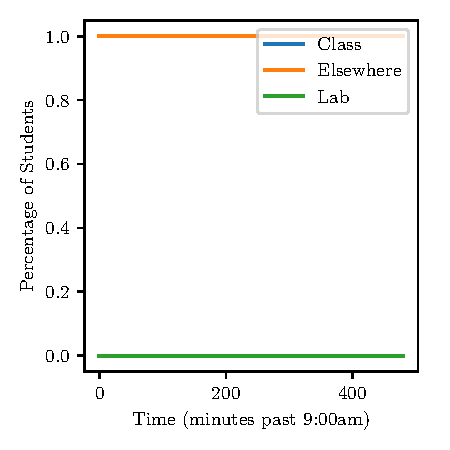
\includegraphics[width=0.45\textwidth]{temp.pdf}\hfill

    \caption{The discontinuous alpha functions (left) along with the timeplot using IVP (right).}
    \label{fig:discontinuous_alpha}

\end{figure}




\begin{figure}[htp]
    \centering
    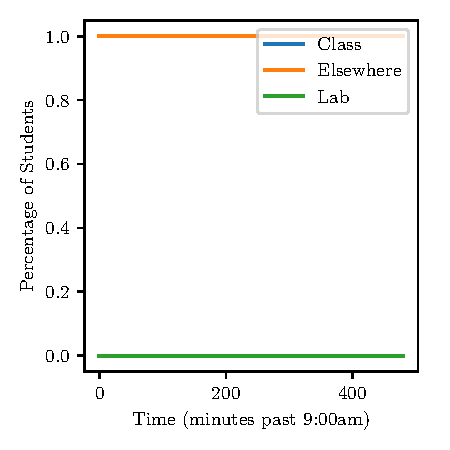
\includegraphics[width=0.3\textwidth]{temp.pdf}\hfill
    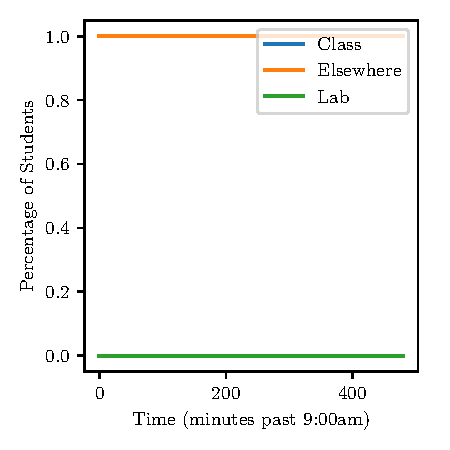
\includegraphics[width=0.3\textwidth]{temp.pdf}\hfill
    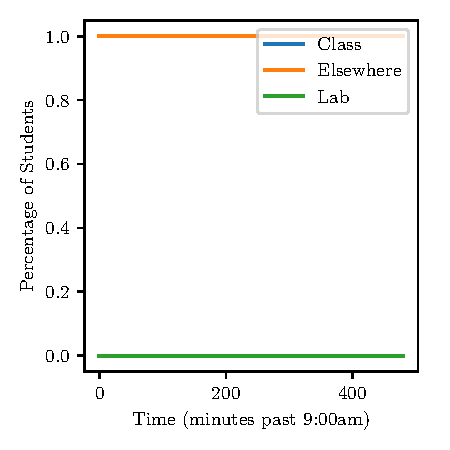
\includegraphics[width=0.3\textwidth]{temp.pdf}\hfill
    \caption{Simulating with $A_{interp.12}$ (left), giving the timeplots using both IVP (center) and BVP (right).}
    \label{fig:continuous_alpha}

\end{figure}









%%%%%%%%%%%%%%%%%%%%%%%%%%%%%%%%%%%%%
%% Bibliography below
%%%%%%%%%%%%%%%%%%%%%%%%%%%%%%%%%%%%%
\FloatBarrier % Keep the figures from being put after the bibliography
\newpage
%% If using bibtex, leave this uncommented
%\bibliography{refs} %if using bibtex, call your bibtex file refs.bib
\bibliographystyle{alpha}

%% If not using bibtex, comment out the previous two lines and uncomment those below
\begin{thebibliography}{99}
\bibitem{Research} G. Kurz, I. Gilitschenski and U. D. Hanebeck, "Recursive nonlinear filtering for angular data based on circular distributions," \textit{2013 American Control Conference}, Washington, DC, USA, 2013, pp. 5439-5445, doi: 10.1109/ACC.2013.6580688.
\bibitem{V3} The ACME Volume 3 Textbook
\bibitem{V3 Lab Manual} J. Humpherys and T. Jarvis, "Labs for Foundations of Applied Mathematics, Volume 3, Modeling with Uncertainty and Data."
\bibitem{Particle} Labbe, Roger. “Kalman and Bayesian Filters in Python”.
\bibitem{Risk} Masson, Maxime; Lamoureux, Julie; de Guise, Elaine (October 2019). "Self-reported risk-taking and sensation-seeking behavior predict helmet wear amongst Canadian ski and snowboard instructors". \textit{Canadian Journal of Behavioural Science.} 52 (2): 121–130. doi:10.1037/cbs0000153. S2CID 210359660.
\bibitem{Oops} I. Marković and I. Petrović, "Speaker localization and tracking with a microphone array on a mobile robot using von Mises distribution and particle filtering," \textit{Robotics and Autonomous Systems}, Volume 58, Issue 11, 2010, pp. 1185-1196, doi: 10.1016/j.robot.2010.08.001
\end{thebibliography}

\end{document}
